\documentclass{beamer}

\usepackage{pgfpages}
\usepackage{caption}
\setbeameroption{show notes on second screen}

\setbeamertemplate{caption}[numbered]
\setbeamerfont{note page}{size=\scriptsize}

\mode<presentation>

\title{Perbandingan Algoritma \textit{Backtracking} dan Algoritma \textit{Hybrid Genetic} untuk Menyelesaikan Permainan Calcudoku}
\author{Michael Adrian \\ 2013730039 \\ \texttt{michaeladrian39@gmail.com}}
\institute{Jurusan Teknik Informatika \\ Fakultas Teknologi Informasi dan Sains \\ Universitas Katolik Parahyangan}
\date{6 Desember 2016}

\begin{document}

\begin{frame}
\titlepage
\end{frame}

\section{Dasar Teori}

\subsection{Calcudoku}

\begin{frame}
\frametitle{Calcudoku}
\begin{definition}
\begin{itemize}
\item Salah satu jenis permainan teka-teki aritmatika dan logika
\item Dikenal juga sebagai KenKen, KenDoku, atau Mathdoku
\item Diciptakan pada tahun 2004 oleh Tetsuya Miyamoto, seorang guru matematika dari Jepang
\item Diciptakan untuk melatih kemampuan matematika dan logika dengan cara yang menyenangkan
\end{itemize}
\end{definition}
\end{frame}

\note{
Sebagai salah satu jenis permainan teka-teki aritmatika dan \textit{grid}, Calcudoku, atau dikenal juga sebagai KenKen, KenDoku, atau Mathdoku, diciptakan pada tahun 2004 oleh seorang guru matematika dari Jepang yang bernama Tetsuya Miyamoto untuk memenuhi tujuannya untuk melatih kemampuan matematika dan logika siswa-siswinya dengan cara yang menyenangkan. Nama KenKen diambil dari kata bahasa Jepang yang berarti kepandaian. Permainan yang mengasah otak ini dengan cepat menyebar ke seluruh Jepang dan Amerika Serikat, menggantikan permainan teka-teki silang di banyak koran. Permainan ini kemudian menjadi sensasi di seluruh dunia setelah munculnya versi \textit{online} dan \textit{mobile} dari permainan teka-teki ini, khususnya menarik untuk pecinta permainan teka-teki angka seperti Sudoku.
}

\begin{frame}
\frametitle{Aturan Permainan}
\begin{itemize}
\item Pemain diberikan sebuah \textit{grid} dengan ukuran \begin{math}n \times n\end{math}
\item \begin{math}n\end{math} biasanya antara 3 sampai dengan 9
\item \textit{Grid} ini harus diisi dengan angka 1 sampai dengan \begin{math}n\end{math}
\item Dalam setiap baris setiap angka hanya muncul sekali
\item Dalam setiap kolom setiap angka hanya muncul sekali
\item \textit{Grid} dibagi ke dalam \textit{cage}
\item \textit{Cage} adalah sekelompok sel yang dibatasi oleh garis yang lebih tebal daripada garis pembatas antar sel dengan angka tujuan dan operator yang telah ditentukan
\item Angka-angka dalam setiap \textit{cage} harus mencapai angka tujuan jika dihitung menggunakan operator yang telah ditentukan
\item Angka tujuan dan operasi yang telah ditentukan ditulis di sudut kiri atas \textit{cage}
\end{itemize}
\end{frame}

\note{
Seperti dalam Sudoku, dalam teka-teki ini, pemain diberikan sebuah \textit{grid} dengan ukuran \begin{math}n \times n\end{math}, dengan \begin{math}n\end{math} biasanya antara 3 sampai dengan 9. \textit{Grid} ini harus diisi dengan angka 1 sampai dengan \begin{math}n\end{math} sehingga dalam setiap baris setiap angka hanya muncul sekali, dalam setiap kolom setiap angka hanya muncul sekali. Perbedaannya dengan Sudoku adalah, Calcudoku dibagi ke dalam \textit{cage} (sekelompok sel yang dibatasi oleh garis yang lebih tebal daripada garis pembatas antar sel dengan angka tujuan dan operator yang telah ditentukan), dan angka-angka dalam setiap \textit{cage} harus mencapai angka tujuan jika dihitung menggunakan operator yang telah ditentukan. Angka tujuan dan operasi yang telah ditentukan ditulis di sudut kiri atas \textit{cage}.
}

\begin{frame}
\frametitle{Operator-Operator Matematika}
\begin{itemize}
\item Ada 5 kemungkinan operator:
	\begin{itemize}
	\item + (penjumlahan)
	\item - (pengurangan)
	\item \begin{math}\times\end{math} (perkalian)
	\item \begin{math}\div\end{math} (pembagian)
	\item = (sama dengan)
	\end{itemize}
\item Jika operasi matematika yang ditentukan adalah pengurangan atau pembagian, maka ukuruan \textit{cage} harus berukuran dua sel
\end{itemize}
\end{frame}

\note{
Ada lima kemungkinan operator:
\begin{enumerate}
\item +, sebuah operator \begin{math}n\end{math}-ary yang menandakan penjumlahan.
\item -, sebuah operator biner yang menandakan pengurangan.
\item \begin{math}\times\end{math}, sebuah operator  \begin{math}n\end{math}-ary yang menandakan perkalian.
\item \begin{math}\div\end{math} sebuah operator biner yang menandakan pembagian.
\item =, (simbol ini biasanya dihilangkan), sebuah operator uner yang menandakan persamaan.
\end{enumerate}
Jika operasi matematika yang ditentukan adalah pengurangan atau pembagian, maka ukuruan \textit{cage} harus berukuran dua sel. Pada beberapa versi dari teka-teki ini, hanya angka tujuan yang diberikan, dan pemain harus menebak operator dari setiap \textit{cage} untuk menyelesaikan teka-tekinya ~\cite{fahda:16:backtracking} ~\cite{johanna:12:hybrid}.
}

\begin{frame}
\frametitle{Permasalahan Utama dalam Menyelesaikan Calcudoku}
\begin{itemize}
\item Untuk menyelesaikan sebuah teka-teki Calcudoku, pemain harus pertama-tama memahami dua permasalahan utama dari teka-teki ini, yaitu:
	\begin{itemize}
	\item Angka-angka mana yang harus dimasukkan ke dalam sebuah \textit{cage}
	\item Dalam urutan apa angka-angka tersebut harus dimasukkan ke dalam sebuah \textit{cage}
	\end{itemize}
\end{itemize}
\end{frame}

\note{
Untuk menyelesaikan sebuah teka-teki Calcudoku, pemain harus pertama-tama memahami dua permasalahan utama dari teka-teki ini, yaitu:
\begin{enumerate}
\item Angka-angka mana yang harus dimasukkan ke dalam sebuah \textit{cage}
\item Dalam urutan apa angka-angka tersebut harus dimasukkan ke dalam sebuah \textit{cage}
\end{enumerate}

Seperti kebanyakan permainan teka-teki angka, cara yang paling mudah untuk menyelesaikan teka-teki ini adalah dengan mengeliminasi angka-angka yang sudah digunakan dan mencoba satu per satu angka yang mungkin (\textit{trial and error}). 
}

\begin{frame}
\frametitle{Tahapan Pengisian Calcudoku}
\begin{itemize}
\item Dalam pengisian teka-teki ini ada dua tahapan, yaitu:
	\begin{itemize}
	\item Mencari \textit{cage} yang hanya berukuran 1 sel
	\item Mencari mencari \textit{cage} yang hanya mempunyai satu kemungkinan kombinasi angka
	\end{itemize}
\end{itemize}
\end{frame}

\note{
Dalam pengisian teka-teki ini ada dua tahapan, yaitu:
\begin{enumerate} 
\item Mencari \textit{cage} yang hanya berukuran 1 sel, karena \textit{cage} ini tidak menghasilkan pertanyaan angka apa dan urutan apa. Tahap ini adalah tahap yang paling jelas. Contoh, pada Gambar~\ref{fig:backtracking1}, \textit{cage} pada sudut kiri atas dan \textit{cage} pada sudut kanan bawah hanya berukuran 1 sel, dan dapat langsung diisi dengan angka tujuannya.
\item Mencari mencari \textit{cage} yang hanya mempunyai satu kemungkinan kombinasi angka, sehingga masalah angka-angka apa yang harus diisi dalam \textit{cage} tersebut terjawab. Contoh, \textit{cage} pada sudut kanan atas mempunyai aturan "3-", artinya angka tujuannya adalah 3 dengan menggunakan operasi pengurangan. Satu-satunya pasangan angka dari himpunan \{1,2,3,4\} yang akan menghasilkan angka 3 saat satu angka dikurangkan dari angka yang lainnya adalah \{1,4\}. Namun masalahnya adalah urutan angka-angka yang harus dimasukkan. Dalam kasus ini, untungnya, sel pada sudut kanan bawah sudah diisi dengan angka 1, maka angka 1 tidak bisa digunakan lagi pada kolom yang paling kanan. Jadi, dengan menggunakan cara eliminasi, sel pada sudut kanan atas harus diisi dengan angka 4 dan sel di sebelah kirinya, yaitu sel pada baris yang paling atas dan kolom ketiga dari kiri, harus diisi dengan angka 1. Hal ini memberikan solusi untuk sel pada baris yang paling atas dan kolom kedua dari kiri, yaitu angka 2, karena angka 2 adalah angka yang belum pernah dipakai dalam baris tersebut. Proses ini berlanjut sampai semua sel dalam \textit{grid} terisi dan menghasilkan solusi pada Gambar~\ref{fig:backtracking2} ~\cite{fahda:16:backtracking}.
\end{enumerate}
}

\begin{frame}
\frametitle{Contoh Permainan}
\begin{figure}
\centering
\captionsetup{justification=centering}
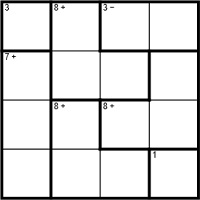
\includegraphics[scale=1]{Gambar/Backtracking1}
\caption[Contoh permainan teka-teki Calcudoku dengan ukuran \textit{grid} 4 x 4 yang belum diselesaikan.  ~\cite{fahda:16:backtracking}]{Contoh permainan teka-teki dengan ukuran \textit{grid} 4 x 4 yang belum diselesaikan.  ~\cite{fahda:16:backtracking}}
\label{fig:backtracking1}
\end{figure}
\end{frame}

\begin{frame}
\frametitle{Contoh Solusi}
\begin{figure}
\centering
\captionsetup{justification=centering}
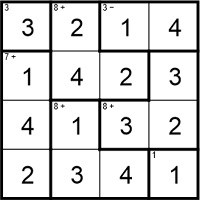
\includegraphics[scale=1]{Gambar/Backtracking2}
\caption[Solusi untuk permainan teka-teki Calcudoku yang diberikan pada Gambar~\ref{fig:backtracking1}  ~\cite{fahda:16:backtracking}]{Solusi untuk permainan teka-teki Calcudoku yang diberikan pada Gambar~\ref{fig:backtracking1}.  ~\cite{fahda:16:backtracking}}
\label{fig:backtracking2}
\end{figure}
\end{frame}

\end{document}